\documentclass{article}
\usepackage{amsmath}
\usepackage{amsthm}
\usepackage{amssymb}
\usepackage{graphicx}
\usepackage{color}
%\include{macros}
%\usepackage{floatflt}
%\usepackage{graphics}
%\usepackage{epsfig}
\usepackage[colorlinks,linkcolor=red,anchorcolor=blue,citecolor=green]{hyperref}
\usepackage{epstopdf}

\usepackage[UTF8]{ctex}
\usepackage{verbatim}
\usepackage[backend=bibtex,style=authoryear,natbib=true,backref=true]{biblatex}

\theoremstyle{definition}
\newtheorem{theorem}{Theorem}[section]
\newtheorem{lemma}[theorem]{Lemma}
\newtheorem{proposition}[theorem]{Proposition}
\newtheorem{corollary}[theorem]{Corollary}

\theoremstyle{definition}
\newtheorem*{definition}{Definition}
\newtheorem*{example}{Example}

\theoremstyle{remark}
\newtheorem*{remark}{Remark}
\newtheorem*{note}{Note}
\newtheorem*{exercise}{Exercise}

\setlength{\oddsidemargin}{-0.25 in}
\setlength{\evensidemargin}{-0.25 in} \setlength{\topmargin}{-0.25
in} \setlength{\textwidth}{7 in} \setlength{\textheight}{8.5 in}
\setlength{\headsep}{0.25 in} \setlength{\parindent}{0 in}
\setlength{\parskip}{0.1 in}

\newcommand{\homework}[4]{
\pagestyle{myheadings} \thispagestyle{plain}
\newpage
\setcounter{page}{1} \noindent
\begin{center}
\framebox{ \vbox{\vspace{2mm} \hbox to 6.28in { {\bf
THU-70250403,~Convex~Optimization~(Fall 2018) \hfill Homework: #4}}
\vspace{6mm} \hbox to 6.28in { {\Large \hfill #1 \hfill} }
\vspace{6mm} \hbox to 6.28in { {\it Lecturer: #2 \hfill} }
\vspace{2mm} \hbox to 6.28in { {\it Student: #3 \hfill} }
\vspace{2mm} } }
\end{center}
\markboth{#1}{#1} \vspace*{4mm} }

\addbibresource{./ref/ref.bib} % The filename of the bibliography

\begin{document}

\homework{L1-TWSVM}{Shuning Wang, Li Li \hspace{5mm} {\tt swang@tsinghua.edu.cn \tt
li-li@tsinghua.edu.cn }}{闫茹钰, 喻望, 张芙作, 郑洁, 朱榕平 \hspace{5mm} {\tt }}{1}

\section{数值实验}

类似论文原文,我们使用\emph{异或问题}测试 L1-TWSVM 算法的正确性。由于异或问题比较简单,直接采用本地随机生成的数据集。本次实验分别以点 $(0,\,0),\, (0,\,1),\, (1,\,0),\, (1,\,1)$ 为中心,范围 $[\pm 0.15,\, \pm 0.15]$ 内均匀产生 10 个样本点;再手动添加两个离群点 $(1.2,\, -0.3),\, (-0.3,\, -0.3)$。得到数据散点图如图 \ref{data_points} 所示。

\begin{figure}[ht]
\centering
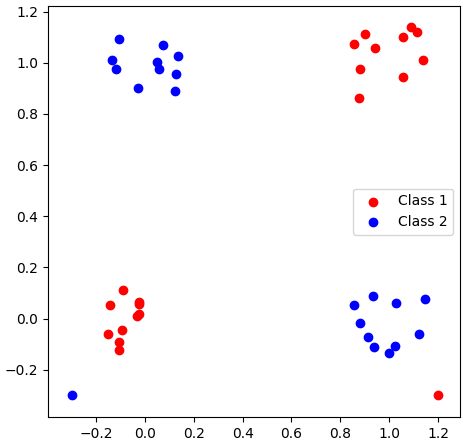
\includegraphics[width=0.35\textwidth]{./img/datas.png}
\caption{数据散点图}
\label{data_points}
\end{figure}

实验代码采用 \verb|Python| 编写,调用 \verb|cvxpy| \parencite{cvxpy} 求解凸优化问题,详细代码见附录 \ref{append_code}。首先不添加离群点,观察 TWSVM 与 L1-TWSVM 拟合超平面的效果对比,得到输出:
\begin{verbatim}
Init solution z1:  [-0.00934916  0.00960656 -0.00173161]
Init solution z2:  [-0.00083704 -0.00064728  0.00173187]
Final solution z1: [-2.1700e-08  2.2172e-08 -4.1194e-09]
Final solution z2: [-2.2670e-09 -1.7231e-09  3.0088e-09]
\end{verbatim}
拟合结果如图 \ref{no_out_no_reg},可见四条拟合直线都存在较大问题。考察优化目标 $\frac{1}{2}\mathbf{z}_1^T \mathbf{H}^T \mathbf{D}_1 \mathbf{H} \mathbf{z}_1 + c_1 \mathbf{e}_2^T \mathbf{q}_1$,由于改变超平面系数比例不会影响超平面的法线方向和位置,所以系数尺度越小,目标函数值越小,所以最优解将会具有较小的模长。但是求解问题时由除法操作,在数值计算中,除以较小数将导致较大的误差,因此造成超平面偏离数据点。直观的解决方法是增加 $\|\mathbf{z}_1\|_2 = 1$ 的约束,但此时问题将变成非凸。所以最后采用 $\mathbf{z}_1^{(1)} = 1$,$\mathbf{z}_1^{(1)}$ 即向量首元素,作为新的约束。修改后得到输出:
\begin{verbatim}
Init solution z1:  [ 1. -1.01312805  0.06991737]
Init solution z2:  [ 1.  0.93863708 -0.95349977]
Final solution z1: [ 1. -0.99892206  0.04902573]
Final solution z2: [ 1.  0.86698756 -0.90293122]
\end{verbatim}
拟合结果如图 \ref{no_out},两个算法结果相近。由于 $l_1$-范数受较远处点的影响较小,所以蓝色直线没有过点集的重心,这也符合预期。

\begin{figure}[ht]
\centering
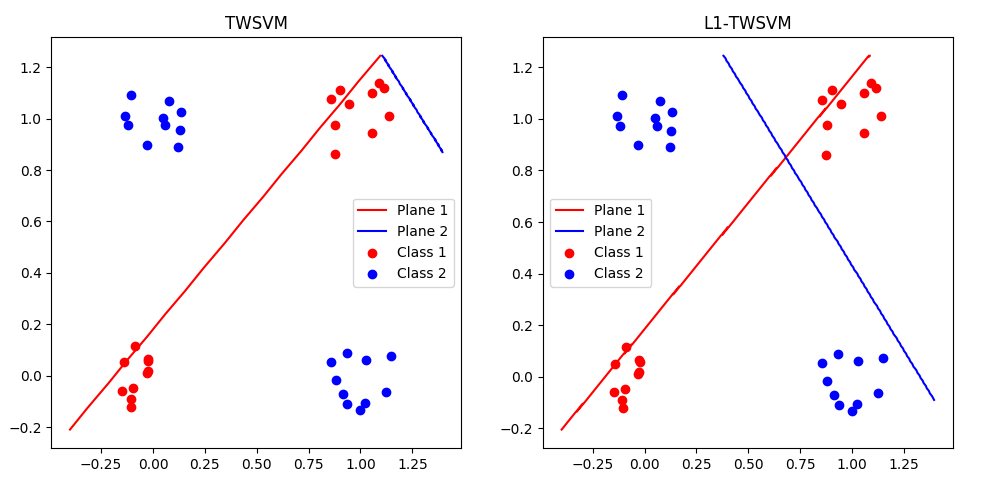
\includegraphics[width=0.8\textwidth]{./img/without_norm_cons.png}
\caption{不带离群点,无参数规范化}
\label{no_out_no_reg}
\end{figure}

\begin{figure}[ht]
\centering
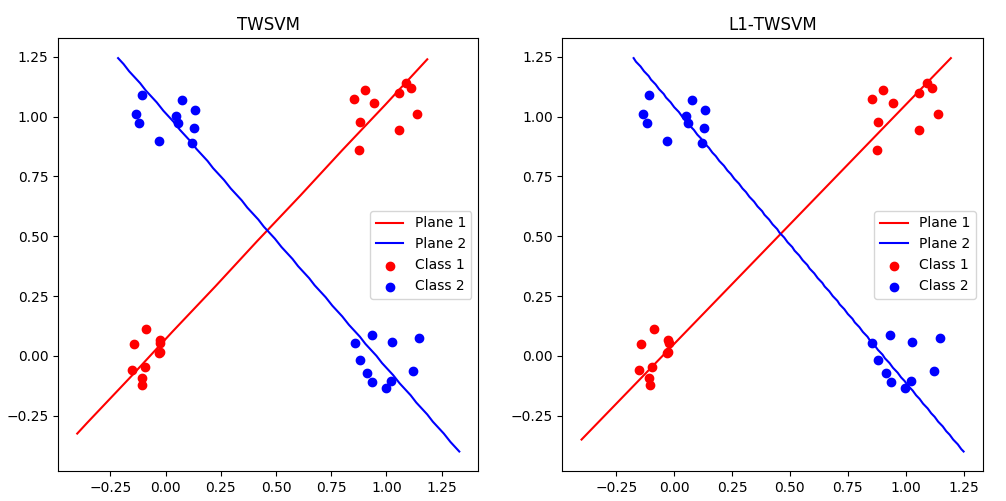
\includegraphics[width=0.8\textwidth]{./img/without_outliers.png}
\caption{不带离群点,参数规范化}
\label{no_out}
\end{figure}

增加离群点再进行实验,拟合结果如图 \ref{outliers}。可见离群点使 $l_2$-范数下的超平面产生较大的偏移,而 L1-TWSVM 拟合的直线受影响较小。实验结果说明,与 TWSVM 相比,L1-TWSVM 确实能够减小离群点对拟合超平面的影响。

\begin{figure}[ht]
\centering
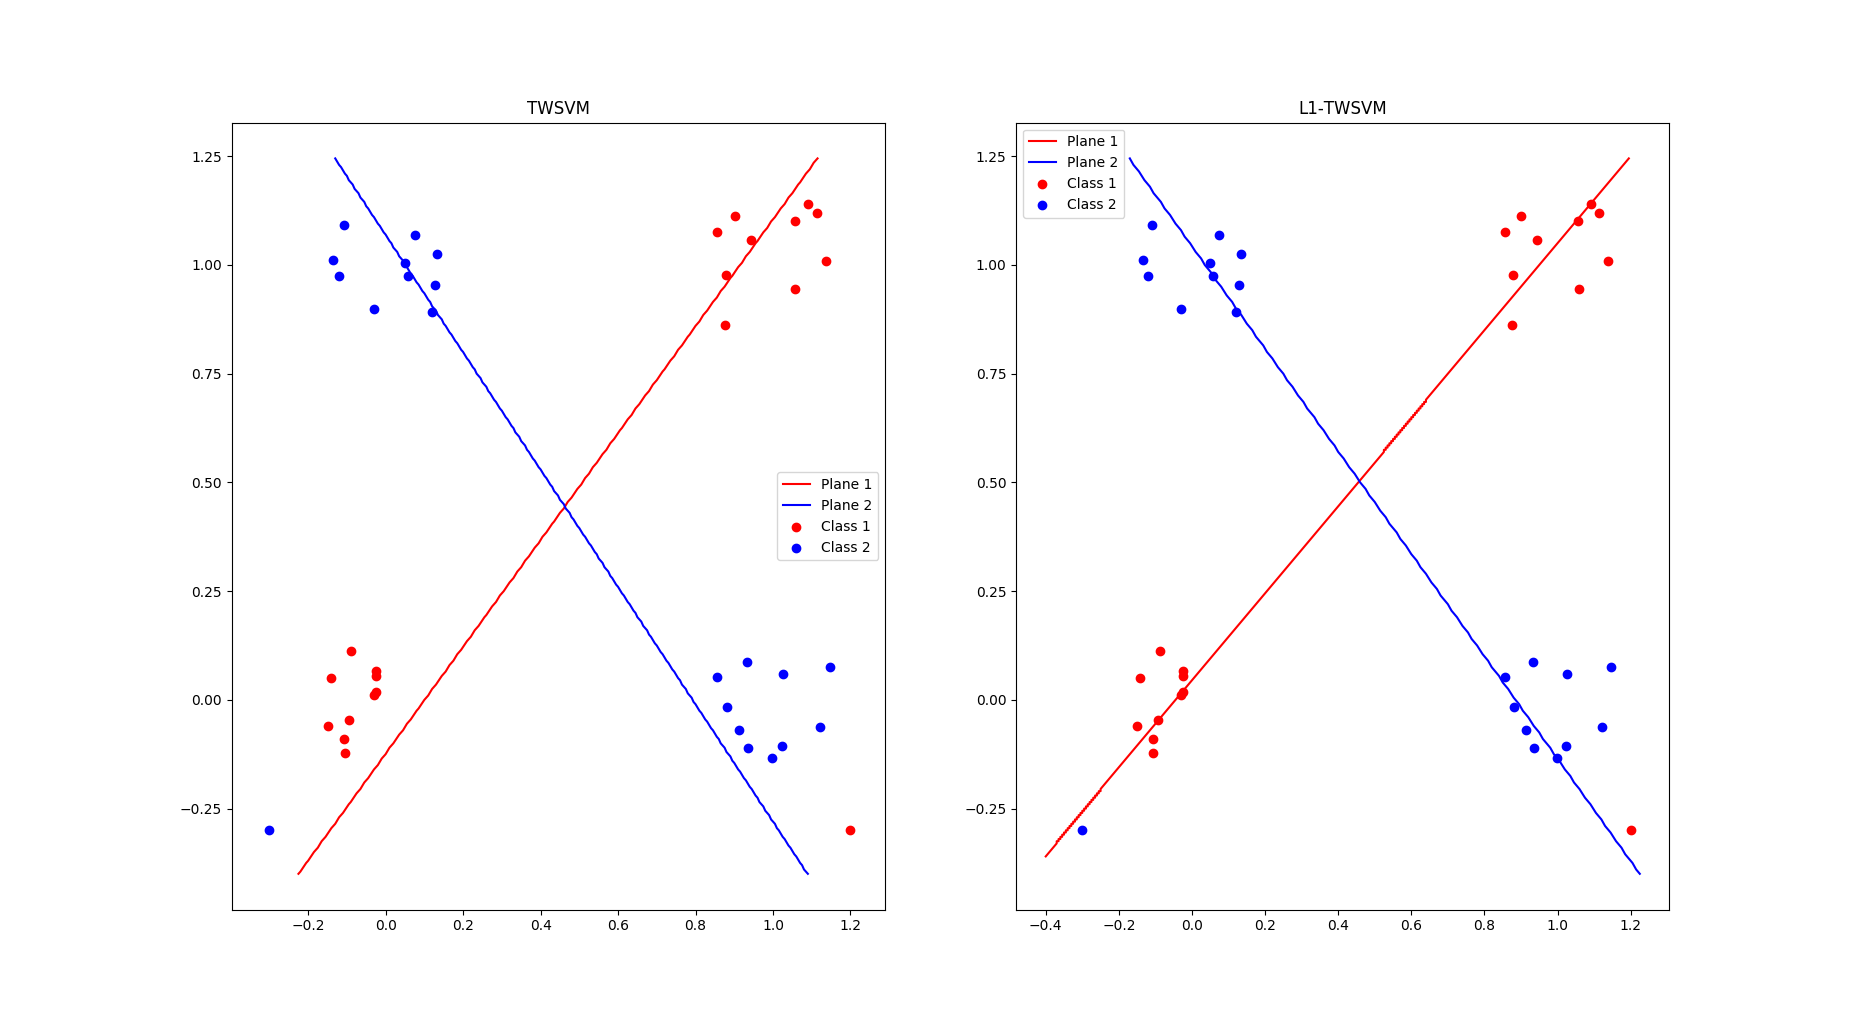
\includegraphics[width=0.8\textwidth]{./img/with_outliers.png}
\caption{带离群点,参数规范化}
\label{outliers}
\end{figure}

\section{总结}

本次作业本组阅读了 \parencite{yan2018efficient},对其中的算法提出思路,算法收敛性证明进行了整理。最后使用 \verb|Python| 进行了数值实验,验证了算法 L1-TWSVM 的正确性。


\printbibliography[heading=bibintoc, title=参考文献]

\appendix
\section{实验代码}
\label{append_code}
\verbatiminput{./codes/main.py}


\end{document}
